\section{Architectural Decisions}
\label{sec:architecture} 

SISDOT is based on the client-server architectural style (according to 
a typical Java enterprise application), where the components interact to each other by requesting 
services from other components~\cite{clements2011documenting}. 
SISDOT is also organized into logical groups of 
components (known as tiers)---a strategy often used in the 
client-server architectural style. The multi-tier architectural pattern 
can be classified as a \emph{component and connector} pattern, 
depending on the criterion used to define the tiers~\cite{bass2013software}. 
Indeed, there are several criteria, such as component type, sharing of the execution environment, 
and so on~\cite{clements2011documenting}.

The multi-tier pattern also induces some topological constraints 
that govern how the components might interact with other components. 
Specifically, connectors might only exist 
between components of the same tier or that reside in an adjacent 
tier~\cite{clements2011documenting}. In addition, according to Bass et al., 
the organization of a system using tiers supports software maintenance, facilitates the definition of 
security policies, and might increase the performance, availability, and modifiability of 
the systems~\cite{bass2013software}. 


\subsection{Runtime Architectural Description}

In order to further detail and illustrate the SISDOT architecture, 
and the main architectural decisions to address the constraints introduced 
in Section~\ref{sec:logistics}, here we present a scenario that refers to the 
generation of QDMs using a runtime architectural 
description (see Figure~\ref{fig:fig:runtime_qdm}). 

%\begin{figure*}
\begin{figure}[!ht] \centering
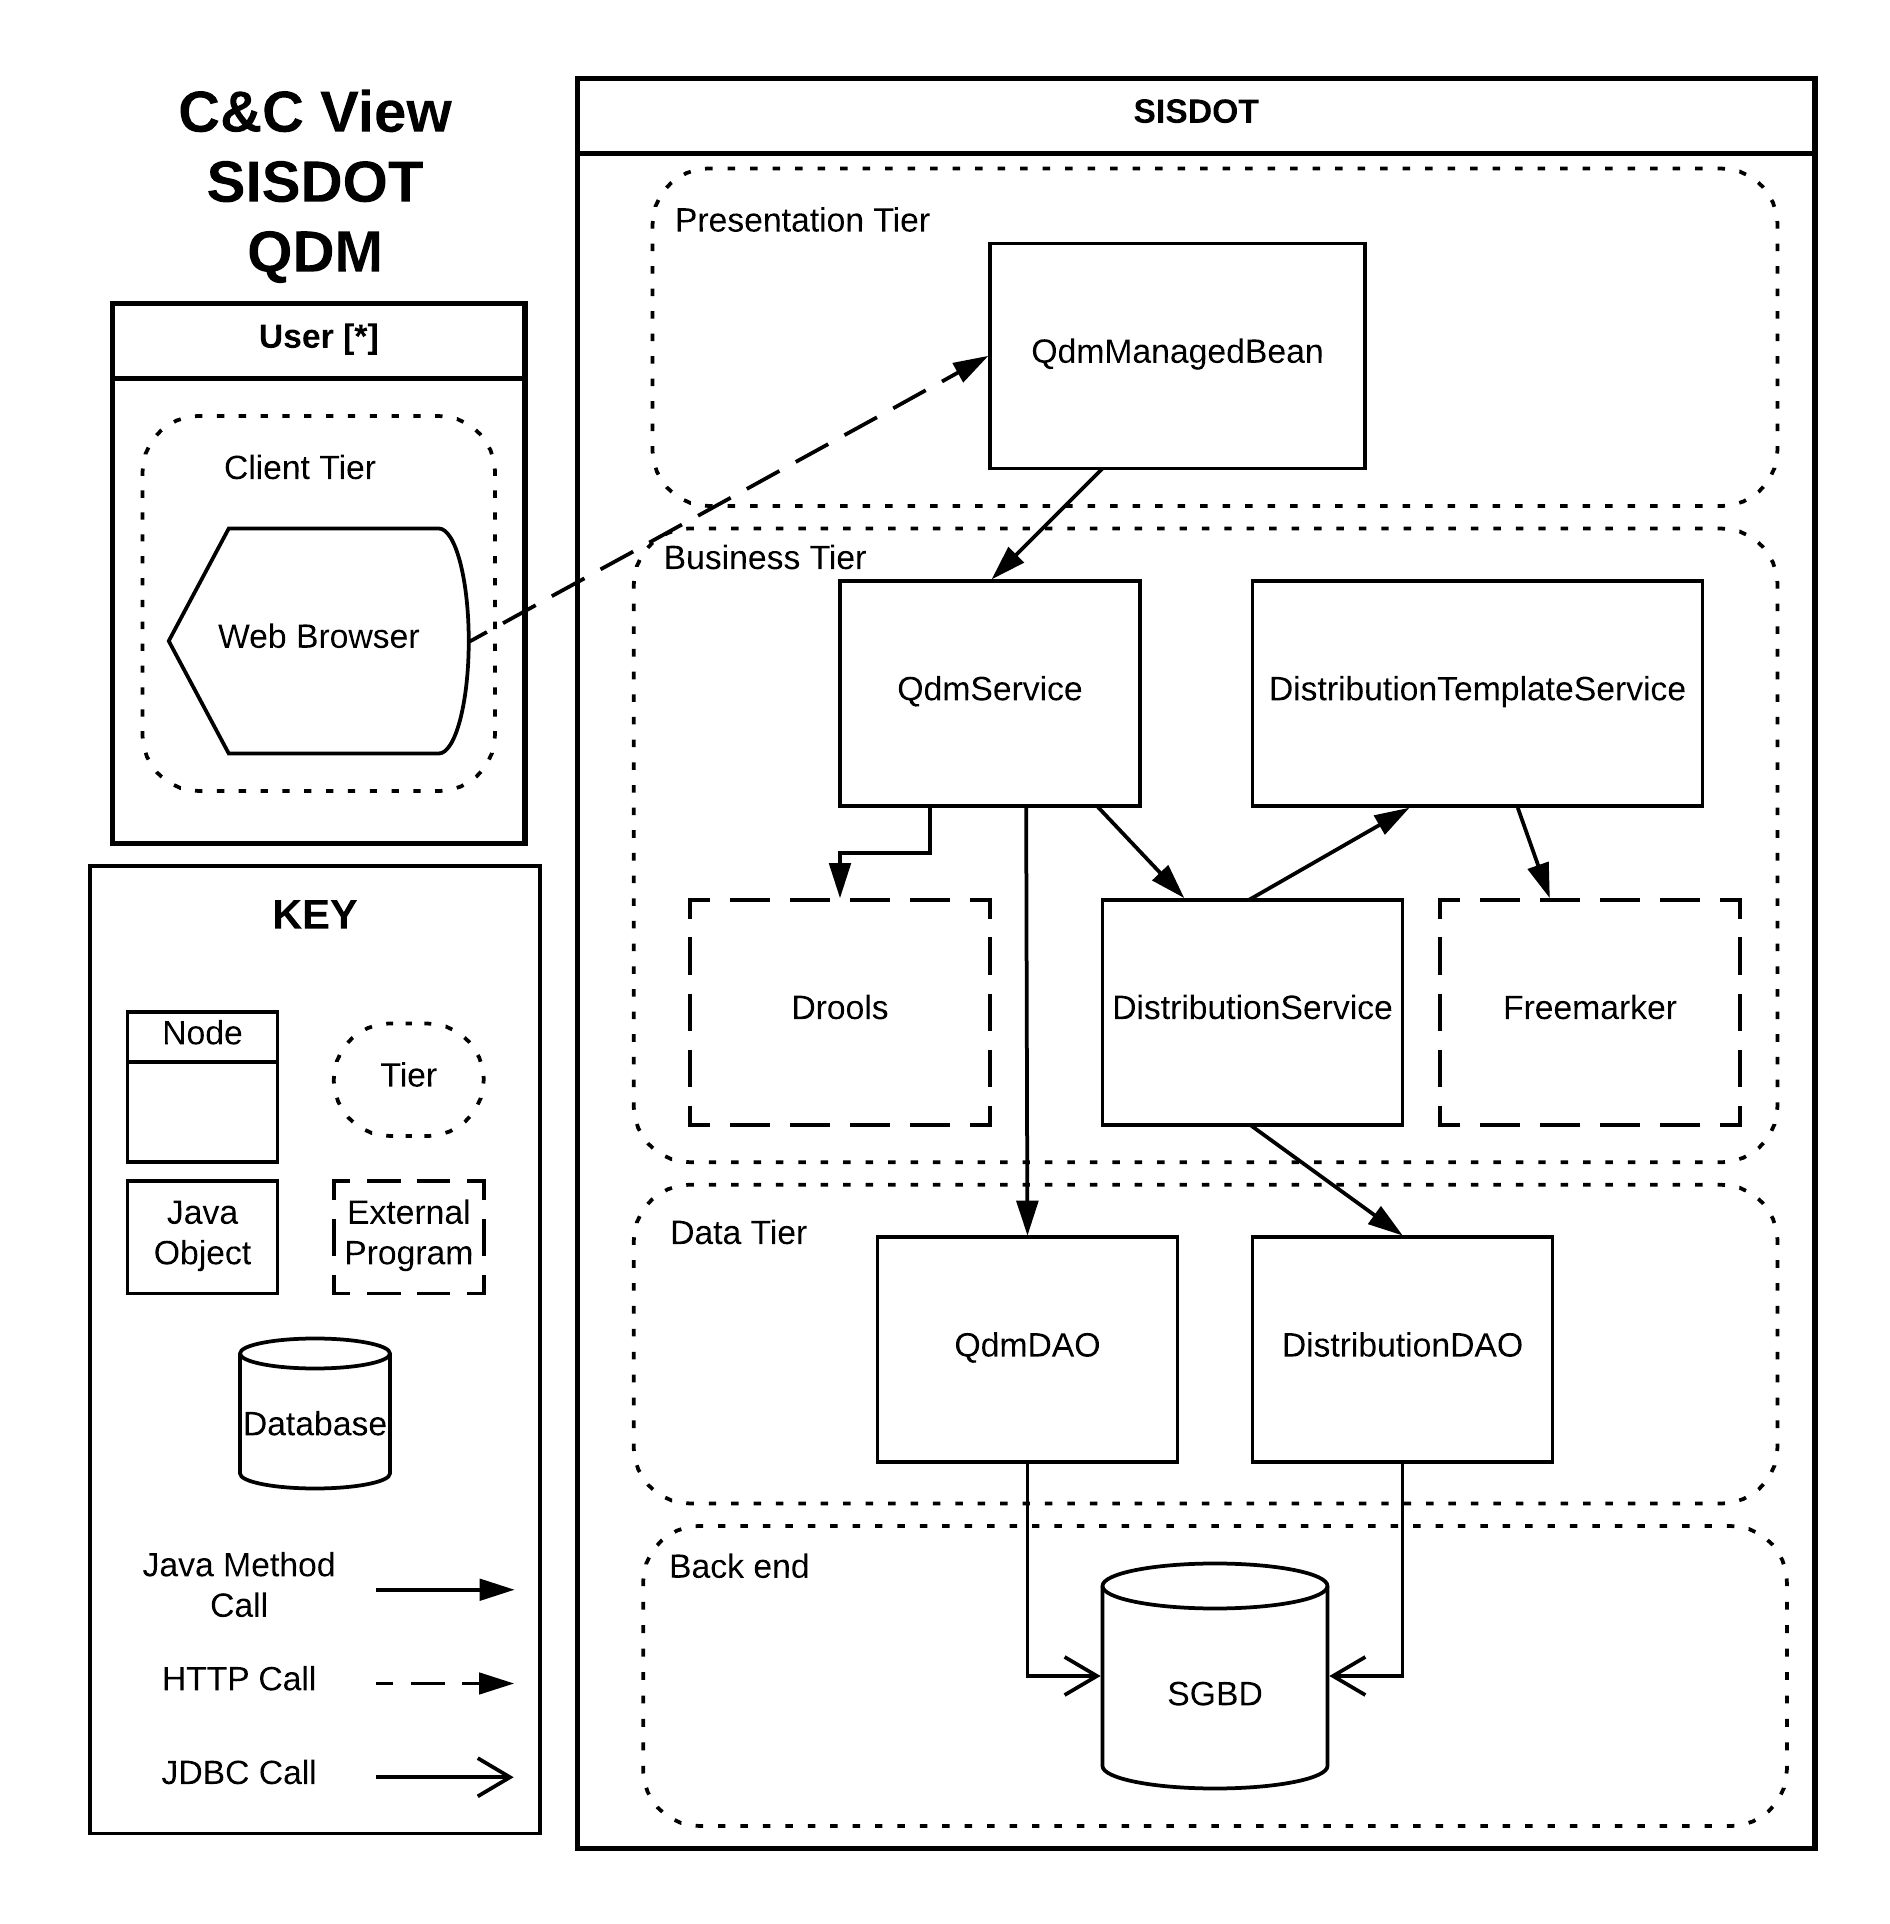
\includegraphics[scale=0.55]{img/runtimeView_qdm.png}
\caption{Runtime view of the architecture} 
\label{fig:fig:runtime_qdm}
\end{figure}
%\end{figure*}

\emph{Considering the user interaction}, a previously authenticated specialist on the 
distribution of equipments throughout the Brazilian Army, using her web browser, 
requests the web page that allows the generation of QDMs (one of the main products of SISDOT). 
After selecting the \emph{generic organizational unity} for which a QDM would be 
generated, the system sends a request to the server. The client tier is responsible for these actions. 
The request is then received by the SISDOT presentation tier, more specifically by a \emph{managed bean} that works 
as a \emph{front controller} (in this case, a JSF controller). 

This controller validates  
the request data, before sending a new request to the business tier. In the business tier, the service 
that implements the business rules related to the QDM domain object is invoked to start the QDM generation process, 
which includes the transformation of \callers into the \emph{low-level rules} specified using the Drools Rule Language (DRL), 
the execution of these rules to instantiate a business object that represents a QDM, and finally saving this 
object in the persistence layer (a relational database). 

The process of generating a QDM is started by retrieving a list of 
previously registered \callers. An \shc, regardless of its type (either based on the 
full structure of the organization or based on its components), 
is related to one or more \emph{military materials / equipments} (MEMs) 
and defines the respective amount that should be assigned to a military 
unit (which ranges from an organization, a center, a department, a brigade, or even 
a military function or qualification of a soldier). 

A low-level rule has one or more distribution rules. Each rule has a type, 
a value, and an associated description. For example, a rule for a 
department type has the value of the department identifier and the description of 
the department name. For a better use of the database, avoiding the definition 
of numerous columns that would inevitably be null for several rule types, we decided 
to persist the distribution rules of an \shc using JSON (JavaScript Object Notation), which is 
converted back to an object when it is retrieved. The set of these rules defines 
exactly who should receive the MEMs specified by the \shc.

% Um dos fatores que motivou o uso de um rule engine foi a similaridade entre chamadores e as regras 'se-então' características destes mecanismos. Um chamador possui um conjunto de condições que se encaixam na parte condicional de uma regra ('se') e possui uma série de ações ('então') que, no caso, são os MEMs que devem ser distribuídos em consequência da validade das condições. A estrutura básica de uma DRL pode ser vista na Listing \ref{code:drlStructure}.

One of the factors that motivated the use of a rule based engine was 
the similarity between \callers and the ``if-then'' rules of these mechanisms.  
%whose essential structure is shown in Listing~\ref{code:drlStructure}.
An \shc has a set of conditions that fit the conditional part of a rule (``if'') 
and has a set of actions (``then'') that, in this case, trigger the distribution 
of MEMs throughout the expected military unities.

%\newpage

%\begin{lstlisting}[frame=single, caption={Structure of a rule specified in Drools}, label={code:drlStructure}]
%rule "name"
%    attributes
%    when
%        LHS
%    then
%        RHS
%end
%\end{lstlisting}


The list of retrieved \callers contains only Java objects. 
In order to be able to use the rule engine in a transparent way for the end users 
(and also for developers in future maintenance scenarios), we decided to use a 
meta-programming approach, translating these objects into a set of rules (i.e., a program in 
logic programming) that might be used by a rule-based engine. As mentioned before,  
we decided to use Drools to support a rule-based engine in the context of 
SISDOT (Figure \ref{fig:fig:runtime_qdm}), mostly because of its integration capabilities 
with both JEE systems and the Wildfly application server. Accordingly,  
the \callers are translated into DRL rules. To this end, we use a template engine (Freemaker) 
to implement this particular transformation (Figure \ref{fig:fig:runtime_qdm}), using a template 
that contains the required \emph{markups} for transforming \shc into \emph{low-level} Drools 
rules. That is, for each \shc, the template engine populates the template, 
resulting in a DRL rule consistent with the converted \shc.
{\color{red}A simplified version of the template used for DRL generation can be seen in} Listing \ref{code:template}.

%\begin{figure}[!ht] \centering
%	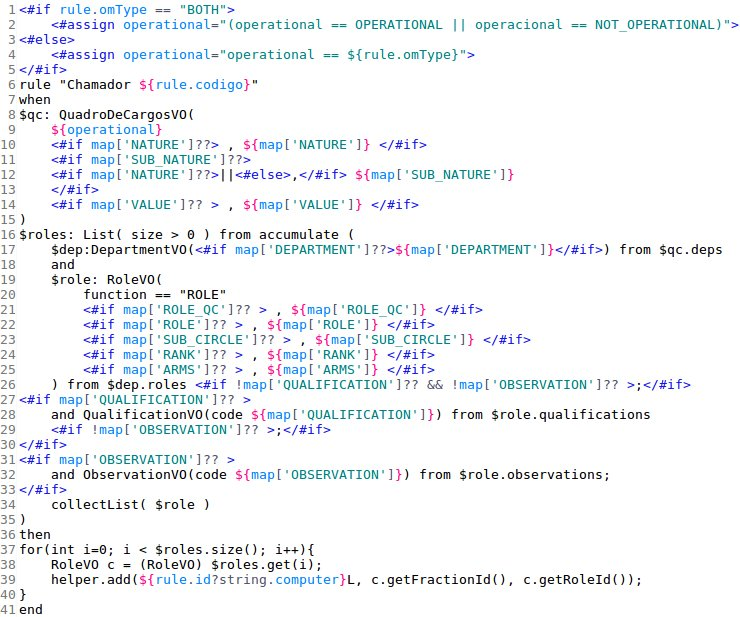
\includegraphics[width=.48\textwidth]{img/artigo_template.jpg}
%	\caption{\it Freemarker template for generating DRL} 
%	\label{fig:template}
%\end{figure}


A QDM is generated for a generic organizational unity (hereafter QC, from \emph{Quadro de Cargos} in Portuguese), 
selected by the user on the client tier. 
Therefore, the user-specified QC must be retrieved from the Brazilian Army's enterprise database  
through a specific Data Access Object (DAO) of the data tier~\cite{alur2003}.
From the list of DRL rules, created based on existing \callers, the rule engine is instantiated and these rules are compiled, 
so that they can be triggered by Drools. The recovered QC is inserted into the working memory as a fact,  an 
information that is considered true. The rules are only executed when their conditions are satisfied, 
based on the specified QC organizational structure. When a rule is valid, that is, it has been activated 
and the \emph{Left Hand Side} (LHS) conditions are valid, 
the QDM is populated with the MEMs specified in the \emph{Right Hand Side} (RHS) of the rules. Therefore, we generate a 
complete QDM object after verifying all valid rules (previously registered in the database) for 
the selected QC. 

\begin{lstlisting}[frame=single, language=Freemarker, caption={\it Freemarker template for generating DRL}, label={code:template},basicstyle=\scriptsize]
<#if rule.omType == "BOTH">
<#assign operational="(operational==OPERATIONAL || operacional==NOT_OPERATIONAL)">
<#else>
<#assign operational="operational==${rule.omType}">
</#if>
rule "Chamador ${rule.codigo}"   	
when
$qc: QuadroDeCargosVO( 
${operational} 				
<#if map['NATURE']??> , ${map['NATURE']} </#if>
<#if map['SUB_NATURE']??>
<#if map['NATURE']??>||<#else>,</#if> ${map['SUB_NATURE']}
</#if>
<#if map['VALUE']?? > , ${map['VALUE']} </#if> 
)	
$roles: List( size > 0 ) from accumulate ( 
$dep:DepartmentVO(<#if map['DEPARTMENT']??>${map['DEPARTMENT']}</#if>) from $qc.deps				  		   
and
$role: RoleVO(
function == "ROLE"
<#if map['ROLE_QC']?? > , ${map['ROLE_QC']} </#if>
<#if map['ROLE']?? > , ${map['ROLE']} </#if>
<#if map['SUB_CIRCLE']?? > , ${map['SUB_CIRCLE']} </#if> 
<#if map['RANK']?? > , ${map['RANK']} </#if>	
<#if map['ARMS']?? > , ${map['ARMS']} </#if>	 										
) from $dep.roles <#if !map['QUALIFICATION']?? && !map['OBSERVATION']?? >;</#if>		
<#if map['QUALIFICATION']?? >
and QualificationVO(code ${map['QUALIFICATION']}) from $role.qualifications 
<#if !map['OBSERVATION']?? >;</#if>	
</#if>				
<#if map['OBSERVATION']?? >
and ObservationVO(code ${map['OBSERVATION']}) from $role.observations;	
</#if>					
collectList( $role )
) 		
then		 
for(int i=0; i < $roles.size(); i++){       	
RoleVO c = (RoleVO) $roles.get(i);
helper.add(${rule.id?string.computer}L, c.getFractionId(), c.getRoleId());       
}               
end
\end{lstlisting}


After the QDM generation, it is saved on the database and we let the domain expert know 
of the success of the operation using a simple user interface message. 
The domain expert can then perform the necessary operations on the generated QDM, including a workflow 
involving  its edition, homologation, and validation.  

\subsection{A DSL for testing the generation of QDMs}

As explained before, to generate a QDM, a set of \callers must be previously 
declared. This is a time-consuming task, particularly when using the interface of 
the system. In order to facilitate the definition of the \callers used in the automated test scripts, we 
decided to create a DSL (Domain Specific Language), enabling us to specify \callers in a 
clear, objective, and declarative way. 

We implemented our DSL using Xtext, which generates plugins that allow editing code in both Eclipse and IntelliJ{, \color{red}plus an editor that can be embedded in a web application}. This way, a developer writing test scripts use our DSL to take advantages of the functionality provided by these plugins.{\color{red} To implement a DSL with Xtext it is necessary to declare a grammar similar to ANTLR \cite{parr2013}, and can be seen in} Listing \ref{code:gramatica}. {\color{red} From the specified grammar Xtext will generate the lexer, the parser, the AST (Abstract Syntax Tree) model, the construction of the AST to represent the parsed program, and the editor with all the IDE features. Xtext comes with good and smart default implementations for all these aspects. However, every single aspect can be customized by the language designer. \cite{bettini2016}.}

%\begin{figure}[!ht] \centering
%	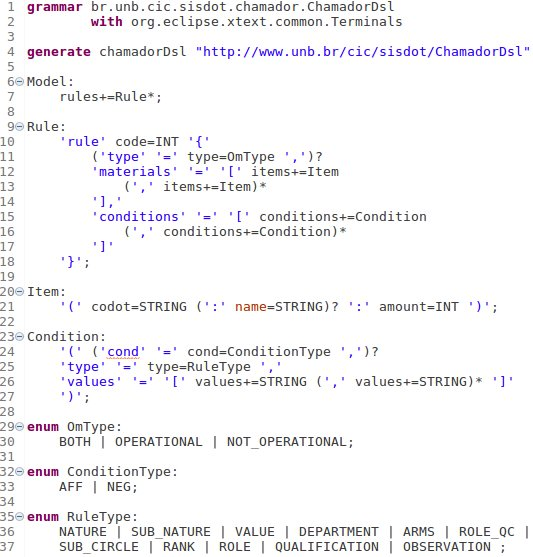
\includegraphics[width=.47\textwidth]{img/artigo_gramatica.jpg}
%	\caption{\it Xtext grammar defining the DSL structure} 
%	\label{fig:gramatica}
%\end{figure}
\begin{lstlisting}[frame=single, language=Xtext, caption={\it Xtext grammar defining the DSL structure}, label={code:gramatica},basicstyle=\scriptsize]
grammar br.unb.cic.sisdot.chamador.ChamadorDsl 
with org.eclipse.xtext.common.Terminals

generate chamadorDsl "http://www.unb.br/cic/sisdot/ChamadorDsl"

Model:
rules+=Rule*;

Rule:
'rule' code=INT '{'
('type' '=' type=OmType ',')?
'materials' '=' '[' items+=Item
(',' items+=Item)*
'],'
'conditions' '=' '[' conditions+=Condition
(',' conditions+=Condition)*
']'
'}';

Item:
'(' codot=STRING (':' name=STRING)? ':' amount=INT ')';

Condition:
'(' ('cond' '=' cond=ConditionType ',')?
'type' '=' type=RuleType ','
'values' '=' '[' values+=STRING (',' values+=STRING)* ']'
')';

enum OmType:
BOTH | OPERATIONAL | NOT_OPERATIONAL;

enum ConditionType:
AFF | NEG;

enum RuleType:
NATURE | SUB_NATURE | VALUE | DEPARTMENT | ARMS | ROLE_QC | SUB_CIRCLE | RANK | ROLE | QUALIFICATION | OBSERVATION ;	\end{lstlisting}

Listing \ref{code:dslExample} presents a simple example of a \shc declaration using our DSL. 
The goal of this rule is to distribute 
the materials (defined in the list of materials construct) for \emph{operational} OMs (see the 
type construct) and militaries \emph{not working in the specified list of 
departments} with a set of qualifications and roles. While the definition of this rule 
using our DSL requires 12 lines of code, the corresponding definition of the same rule 
using a Java test case requires more than 50 lines of imperative code.

\begin{small}
\begin{lstlisting}[frame=single, language=DSL, caption={\it Example of a \shc declaration using our DSL}, label={code:dslExample}]
rule 1 { 
 type = OPERATIONAL, 
 materials = [ 
   ("XXX" : "Rifle" : 1), 
   ("XXY" : "Rifle Carrying Case" : 2)
 ], 
 conditions = [ 
  (cond=NEG, type=DEPARTMENT, values=[...]),
  (type=QUALIFICATION, values=[...]), 
  (type=ROLE, values=[...])
 ]
}
\end{lstlisting}
\end{small}


A test activity consists first in the specification of the required \callers in a file. Next, the \emph{behavior under 
test} is detailed as features using the Cucumber~\cite{wynne2017cucumber} framework (we present an 
example of a feature in Listing \ref{code:cucumber}). After that, the developer details 
the implementation steps of the features by (a) specifying which \callers (previously declared using our DSL) should be considered 
in the test execution, (b) specifying which QC the QDM should be generated, and (c) specifying the expected results in terms 
of the properties of the expected QDM. 

The structure created supports several operations, with the intention 
of increasing the productivity of the tester, such as: database connectivity, auxiliary methods for executing queries 
in the database, and rules in the rule engine. To facilitate the execution even in continuous integration 
environments, we use a maven configuration file that declares the Xtext plugin, responsible for 
generating the necessary code from the DSL, and a plugin for running unit tests (such as surefire).


Altogether, our DSL simplifies the process of specifying \callers. Its primary goal was to 
assist in test activities, though we presented some examples of \callers specified using 
our DSL to domain experts, and they also considered this domain specific language relevant 
to simulate the specification of rules in order to better understand the effect of each 
\shc for building QDMs. Now we are working on a custom user interface for SISDOT to enable domain 
expert to use this specific feature. 


 {\color{red}A DRL gerada para o chamador da Listing \ref{code:dslExample} pode ser vista na} Listing \ref{code:drl}.  {\color{red} Na parte RHS da regra, há uma iteração sobre todos os cargos selecionados. Para cada cargo uma classe que auxilia o preenchimento do QDM é chamada para que os itens declarados no chamador, passado como parâmetro, sejam disponibilizados para o cargo. Essa classe auxiliar recupera o chamador passado como parâmetro a partir da lista de chamadores declarados na DSL, que foram convertidos em objetos Java. Além de auxiliar no preenchimento do QDM, esta classe popula alguns objetos que facilitam a verificação da consistência do QDM, por exemplo.}

%\begin{figure}[!ht] \centering
%	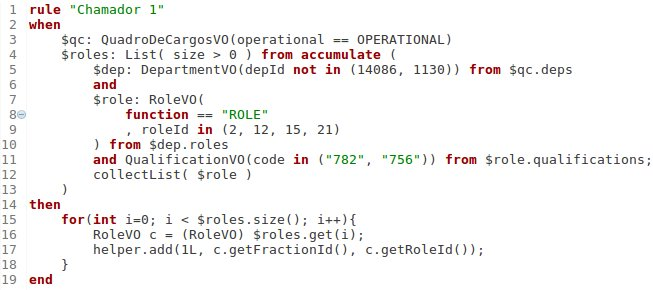
\includegraphics[width=.48\textwidth]{img/artigo_drl.jpg}
%	\caption{\it DRL generated} 
%	\label{fig:drl}
%\end{figure}
\begin{lstlisting}[frame=single, language=DRL, caption={\it DRL generated}, label={code:drl}, basicstyle=\scriptsize]
rule "Chamador 1"   	
when
	$qc: QuadroDeCargosVO(operational == OPERATIONAL)	
	$roles: List( size > 0 ) from accumulate ( 
		$dep: DepartmentVO(depId not in (14086, 1130)) from $qc.deps				  		   
		and
		$role: RoleVO(
			function == "ROLE"
			, roleId in (2, 12, 15, 21)  
		) from $dep.roles 		
		and QualificationVO(code in ("782", "756")) from $role.qualifications;				
		collectList( $role )
	) 		
then		 
	for(int i=0; i < $roles.size(); i++){       	
		RoleVO c = (RoleVO) $roles.get(i);
		helper.add(1L, c.getFractionId(), c.getRoleId());   
}               
end	\end{lstlisting}


We are also working on the automatic generation of test cases 
from our DSL. This effort involves a custom Maven plugin that currently generates simple test cases, 
freeing the tester to create only complex tests related to the QDM generation. 
These test cases are generated from a combination of conditions, for example: one test case only for operational OMs 
and another for non-operational OMs; a test case for each OM nature, combining with the operational type, 
such as: infantry operational OMs and non-operational infantry OMs. These combinations are generated for simple 
cases so that they are easy to verify without the need to build a Java solution for generating QDMs. 


%\begin{figure}[!ht] \centering
%  \includegraphics[width=.32\textwidth]
%  {img/plugin.jpg}
%  \caption{\it Maven plugin for test generation}
%  \label{fig:pluginExample}
%\end{figure}
\begin{lstlisting}[frame=single, language=Plugin, caption={\it Maven plugin for test generation}, label={code:plugin}]
<plugin>
  <groupId>xxx</groupId>
  <artifactId>xxx</artifactId>
  <executions>
    <execution>
      <id>execute</id>			
      <configuration>
        <seed>10</seed>				
        <qcs>702311,762314,575311</qcs>				
      </configuration>
      <goals>
        <goal>generate</goal>
      </goals>
    </execution>
  </executions>
</plugin>	
\end{lstlisting}



%\begin{figure}[!ht] \centering
%  \includegraphics[width=.45\textwidth]
%  {img/artigo_cucumber.jpg}
%  \caption{\it Cucumber feature}
%  \label{fig:cucumber}
%\end{figure}
\begin{lstlisting}[frame=single, language=Cucumber, caption={\it Cucumber feature}, label={code:cucumber}]
Feature: QDM 757311
	As a user
	I want to generate a QDM from HLRs

	Scenario: Test 1
		Given QC with code 757311
		And HRL: 1, 2
		When I generate a QDM
		And the results are consistent
		Then positions must be populated
		| idDep    | idPos   | codot      | amount |
		| 6765748  | 10403   | 1051000025 | 1      |
		| 6765748  | 10403   | 1020100017 | 1      |
		| 6765748  | 10403   | 1020100013 | 1      |
		| 6765748  | 10403   | 1051000006 | 1      |
		| 6765748  | 21328   | 1051000025 | 1      |
		| 6765750  | 10122   | 1051000025 | 1      |    
		| 6765793  | 13276   | 1051000025 | 6      |
		| 6765796  | 24655   | 1051000025 | 1      |
		| 6765796  | 24429   | 1051000025 | 2      |
		| 6765798  | 24429   | 1051000025 | 3      |
		| 6765798  | 11433   | 1051000025 | 9      |   
		And the final result must be:
		| codot      | amount |
		| 1020100013 | 74     |
		| 1020100017 | 74     |
		| 1051000006 | 74     |
		| 1051000025 | 74     |

	Scenario: Test 2
		Given QC with code 757311
		And HRL: 1, 2, 3
		When I generate a QDM
		And the results are inconsistent    
\end{lstlisting}

For each of the possible combinations, we generate a \shc that meets the conditions 
and a cucumber feature that exercises the \shc and compares the expected results declared in the feature. 
Each \shc is considered during the generation of the QDM to the QCs specified in the 
maven plugin. That is, to use this architecture characteristic (here we consider testability as an 
architecture concern), we ``feed'' the maven plugin with a list of QC codes for which the QDMs should be generated, 
besides other optional information, which have default values, such as: connection string for the database, 
seed to be used in the random selection of values within a combination (e.g., considering "20" natures of 
organizational units, randomly take 5 for generating the set of combinations), and the output directory 
where the code should be exported. A basic example of the plugin declaration, omitting some details like 
\texttt{groupId} and \texttt{artifactId}, can be seen in Listing \ref{code:plugin}.

After running the plugin, with the generated code, the tests are executed in a similar way to the test 
definitions detailed before. The tests run along with the other unit tests declared, 
whether DSL-based or not.
